\section{Py Serial}

	\subsection{Python}
	Python adalah bahasa pemrograman yang dibuat oleh Guido van Rossum dan populer sebagai bahasa pemrograman scripting dan Web. Mengacu pada ide wikipedia, Python adalah bahasa pemrograman interpretatif multiguna dengan filosofi desain yang berfokus pada keterbacaan kode. 
	Python dikenal sebagai bahasa pemrograman yang menggabungkan nilai nilai kapabilitas, kemampuan, dengan sintaks kode yang sangat begitu jelas, dan dilengkapi dengan fungsi penyimpanan standar yang menjadikannya komprehensif dan komprehensif. 
	Python mendukung pemrograman multi-paradigma, khususnya, tetapi tidak terbatas, pada pemrograman berorientasi objek, pemrograman imperatif, dan pemrograman fungsional. 
	Python memiliki salah satu fitur yang sangat unik yaitu sebagai bahasa pemrograman dinamis yaitu yang datang dengan manajemen memori otomatis. Seperti bahasa 
	pemrograman dinamis lainnya, python umumnya digunakan sebagai bahasa scripting meskipun dalam prakteknya penggunaan bahasa ini lebih luas termasuk konteks penggunaan yang umumnya tidak dilakukan menggunakan bahasa scripting. 
	Python dapat digunakan untuk berbagai tujuan pembuatan perangkat lunak atau pun pengembangan perangkat lunak dan dapat dijalankan di berbagai platform sistem operasi. Python adalah salah satu contoh bahasa tingkat tinggi. 
	Contoh lain dari bahasa high-rise adalah pascal, c ++, perl, java, dan seterusnya. Sedangkan bahasa tingkat rendah adalah bahasa mesin atau bahasa assembly. 
	Secara sederhana. komputer hanya dapat menjalankan program yang ditulis dalam bahasa mesin. Karena itu. jika sebuah program ditulis dalam bahasa tinght yang tinggi. maka program tersebut harus diolah terlebih dahulu sebelum dapat dijalanlon di komputer. 
	Ini adalah salah satu kekurangan bahasa tingkat tinggi yang membutuhkan waktu untuk memproses suatu program sebelum dijalankan. Namun, bahasa tingkat tinggi memiliki banyak kelebihan. Bahasa tinglrat yang tinggi mudah dipelajari. mudah ditulis. mudah dibaca. dan tentu saja mudah menemukan kesalahan. Bahasa tingkat tinggi juga mudah dibawa untuk dicocokkan dengan mesin yang menjalankannya. 
	
	\subsection{Komunikasi Serial}
		Langkah - langkah untuk melakuan komunikasi serial adalah sebagai berikut :
		
		\begin{enumerate}
			\item Open Phyton Shell
			
				\begin{figure}[ht]
			\centerline{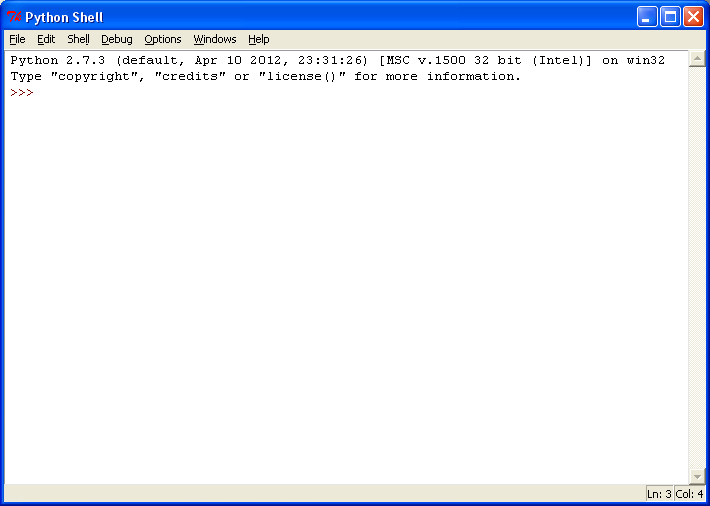
\includegraphics[width=0.5\textwidth]{figures/pyshell.png}}
			\caption{Python Shell}
			\label{pyshell}
			\end{figure}
			
			\item Buat new window seperti atau bisa juga dengan (Ctrl + N), agar muncul window baru.
				
				\begin{figure}[ht]
			\centerline{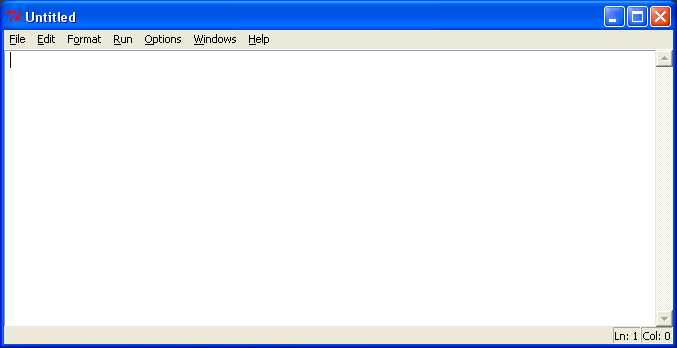
\includegraphics[width=0.5\textwidth]{figures/pyshellnew.png}}
			\caption{New Window}
			\label{pyshellnew}
			\end{figure}
			
			\item Copykan atau ketikkan script ini :
				\begin{verbatim}
					    import serial
						ser = serial.Serial(‘com10’,9600,timeout=1)
						from Tkinter import *
						root=Tk()
						def task():
						a=ser.readline(1)
						print “nilai= ” + a
						root.after(200,task)
						root.after(200,task)
						root.mainloop()
					\end{verbatim}
					
			\item Dibawah ini adalah hasilnya :
			akan muncul window:
			
			\begin{figure}[ht]
			\centerline{
\includegraphics[width=0.5\textwidth]{figures/tkser.png}}
			\caption{TK Window}
			\label{tkser}
			\end{figure}
			
			dan di Python Shell akan muncul :
			
			\begin{figure}[ht]
			\centerline{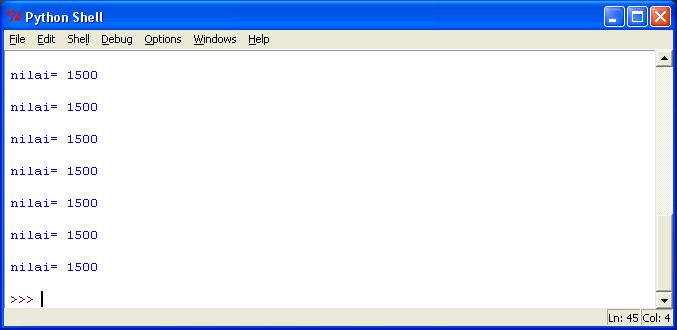
\includegraphics[width=0.5\textwidth]{figures/tkpython.png}}
			\caption{TK Window}
			\label{tkpython}
			\end{figure}
			
		\end{enumerate}
		
		Penjelasannya : 
		\begin{itemize}
			\item import serial
			bagian diatas ini mempunyai fungsi untuk melibatkan module serial sehingga dapat digunakan pada Python.
			
			\item \begin{verbatim} ser = serial.Serial(‘com10’,9600,timeout=1)\end{verbatim}
			Bagian diatas ini berfungsi sebagai pendeklerasian variabel ser sebagai serial port yang propertinya adalah konfigurasi nomer port= COM10, baudrate= 9600, dan timeout=1.
			\item \begin{verbatim} a=ser.readline() \end{verbatim}
			Bagian diatas ini berfungsi untuk membaca data dari serial lalu menampungnya pada variabel a sebagai buffer.
			\item \begin{verbatim} print “nilai= ” + a \end{verbatim} 
			Bagian diatas ini berfungsi untuk tampilkan nilai yang didapat di Python Shell. 
			\item \begin{verbatim} root.after(200,task) \end{verbatim}
			Bagia di atas ini berfungsi untuk melakukan suatu schedule setiap 200 milidetik.
			\item \begin{verbatim} root.after(200,task)	\end{verbatim}
			Bagian diatas ini berfungsi untuk mengulang suatu schedule setiap 200 milidetik.
			\item \begin{verbatim} root.mainloop() \end{verbatim}
			Bagian diatas ini berfungsi untuk melakukan perulangan atau loop.
		\end{itemize}
	
		
